% Chapter Template

\chapter{Results} \label{c4} % Main chapter title

In this chapter, the time it takes to compute each survey statistics with {\bf svydb} will be tested against the {\bf survey} package, both data sets in memory (local) and in database will be used for {\bf svydb}. Up to two million observations was tested with data sets in memory and up to four million observations for data sets in a data base, data set used was The National Health and Nutrition Examination Survey.\\

All computation was done with the same computer, specs as follows,
\begin{itemize}
    \item {\bf MacBook Pro Early 2015}
    \item {\bf Processor} 2.7 GHz Intel Core i5 
    \item {\bf Memory} 8 GB 1867 MHz DDR3
    \item {\bf Graphics} Intel Iris Graphics 6100 1536 MB
\end{itemize}

\hfill

Data sets from 250,000 to 2,000,000 observations were tested on functions which computes replicate survey statistics, up to 4,000,000 observations for other survey statistics and graphics. For all the times, please refer to Appendix \ref{AppendixA}.\\

Legend on graphs corresponds to,
\begin{itemize}
    \item {\bf survey} - {\bf survey} package on local data sets.
    \item {\bf svydb.local}  -  {\bf svydb} on local data sets.
    \item {\bf svydb.database} -  {\bf svydb} package on data sets stored in a database.
\end{itemize}




\section{Total}
\subsection{Numeric variable}
\begin{figure}[H]
    \centering
    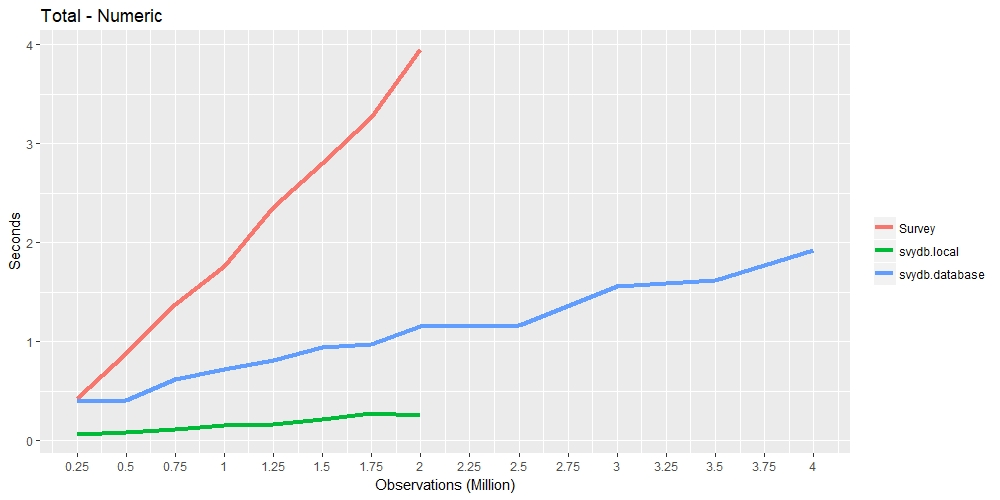
\includegraphics[scale = 0.6]{Latex/img/totnum-r.jpeg}
    \caption{Population total time comparison - Numeric}
    \label{fig:totnum-r}
\end{figure}

\subsection{Categorical variable with 7 levels}

\begin{figure}[H]
    \centering
    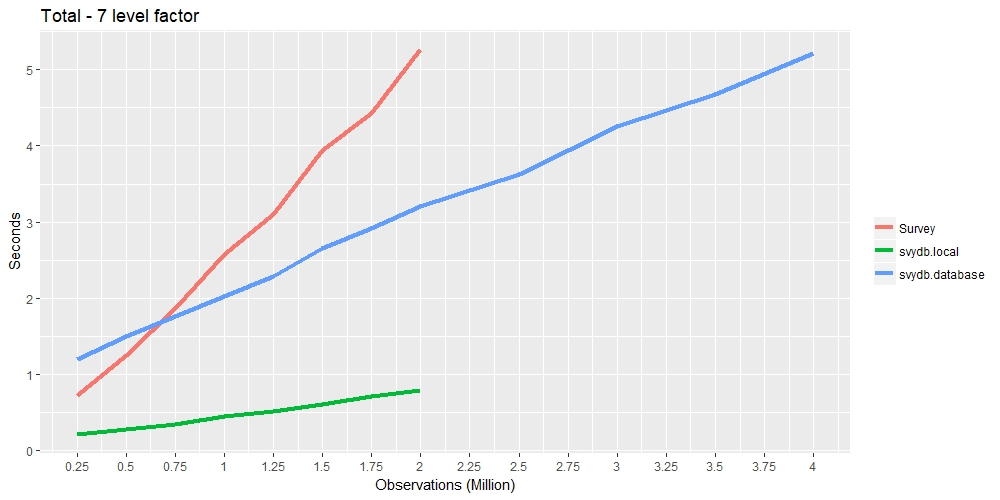
\includegraphics[scale = 0.6]{Latex/img/totcat-r.jpeg}
    \caption{Population total time comparison - Categorical}
    \label{fig:totcat-r}
\end{figure}

%--------------------------------------------------------------------------------------
\section{Mean}
\subsection{Numeric variable}
\begin{figure}[H]
    \centering
    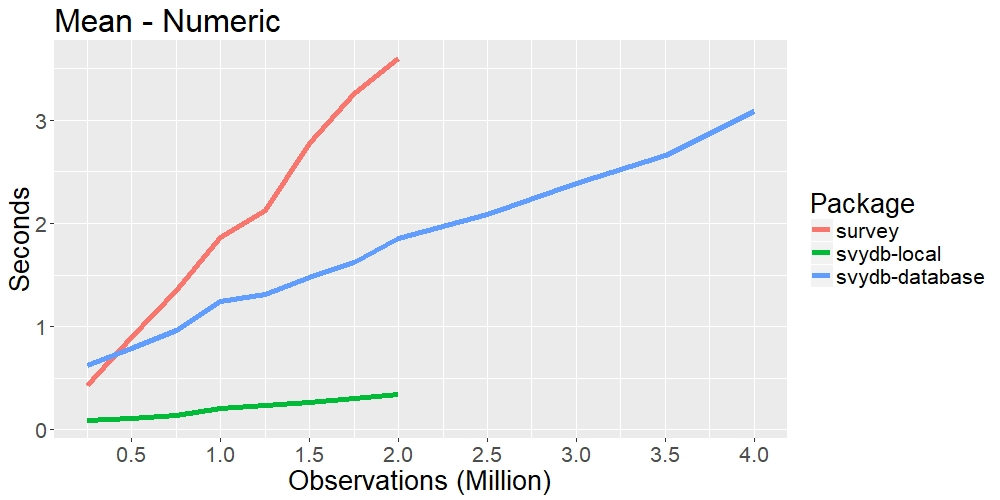
\includegraphics[scale = 0.6]{Latex/img/meannum-r.jpeg}
    \caption{Population mean time comparison - Numeric}
    \label{fig:meannum-r}
\end{figure}

\subsection{Categorical variable with 7 levels}
\begin{figure}[H]
   \centering
    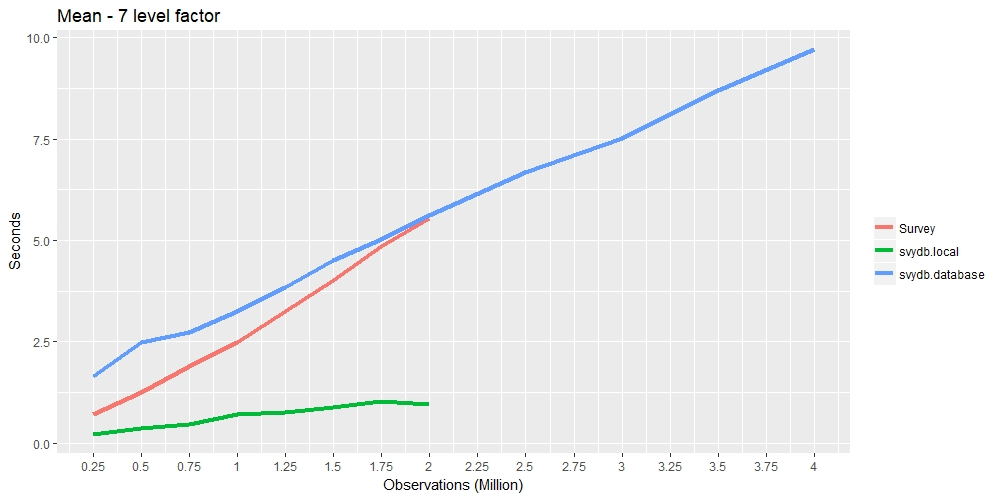
\includegraphics[scale = 0.6]{Latex/img/meancat-r.jpeg}
    \caption{Population mean time comparison - Categorical}
    \label{fig:meancat-r}
\end{figure}

 

%--------------------------------------------------------------------------------------
\section{Regression}
\begin{figure}[H]
   \centering
    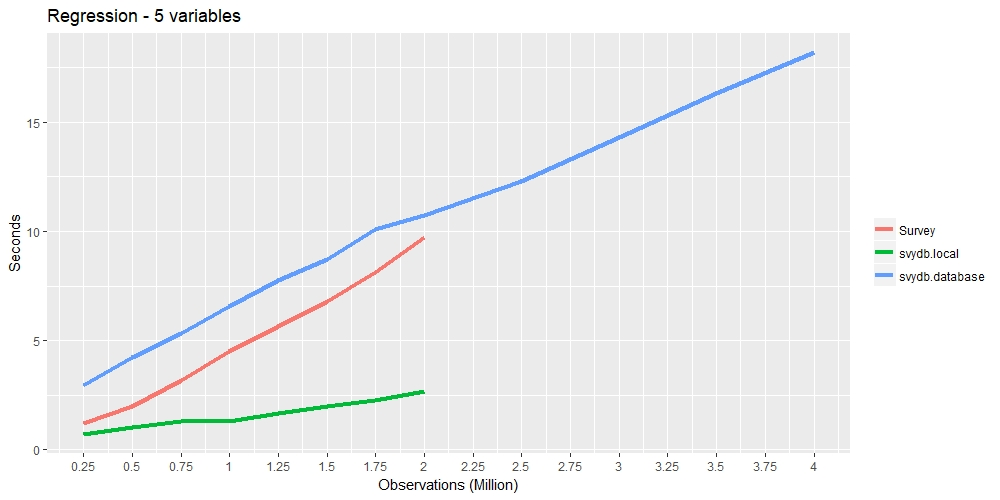
\includegraphics[scale = 0.6]{Latex/img/lm-r.jpeg}
    \caption{Regression time comparison - 5 variables}
    \label{fig:lm-r}
\end{figure}
%--------------------------------------------------------------------------------------
\section{Quantiles}
\begin{figure}[H]
   \centering
    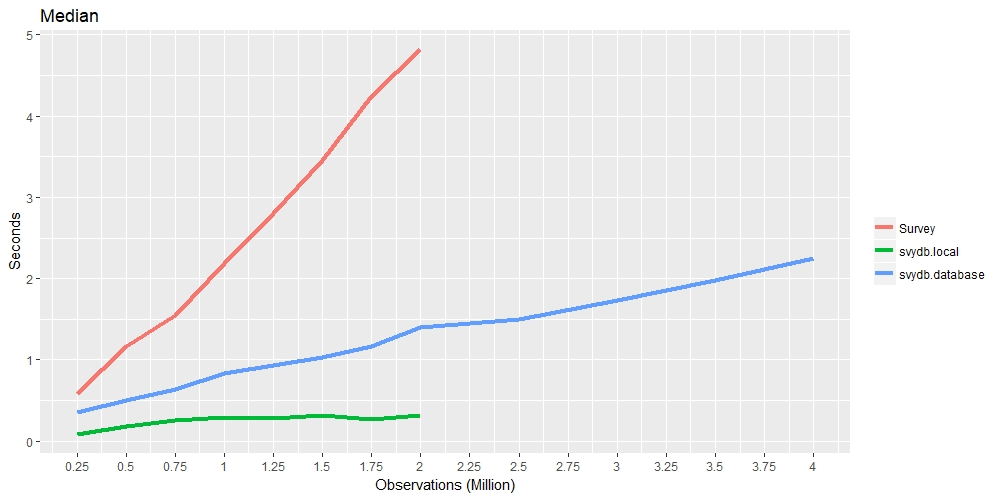
\includegraphics[scale = 0.6]{Latex/img/quantile-r.jpeg}
    \caption{Median time comparison - Categorical}
    \label{fig:quantile-r}
\end{figure}
%--------------------------------------------------------------------------------------
\section{Survey Tables}
\begin{figure}[H]
   \centering
    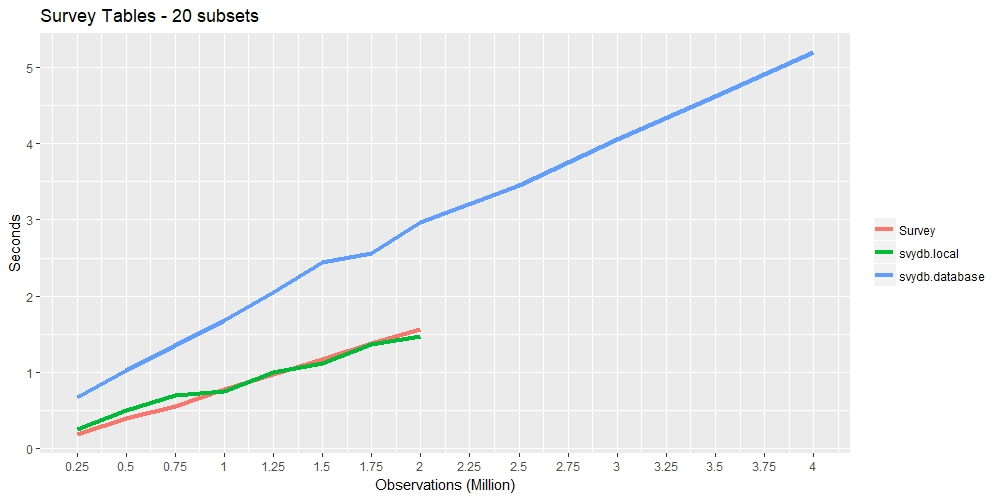
\includegraphics[scale = 0.6]{Latex/img/table-r.jpeg}
    \caption{Tables time comparison - Categorical}
    \label{fig:table-r}
\end{figure}




%--------------------------------------------------------------------------------------
\section{Total - Replicate Weights}
\begin{figure}[H]
  \centering
    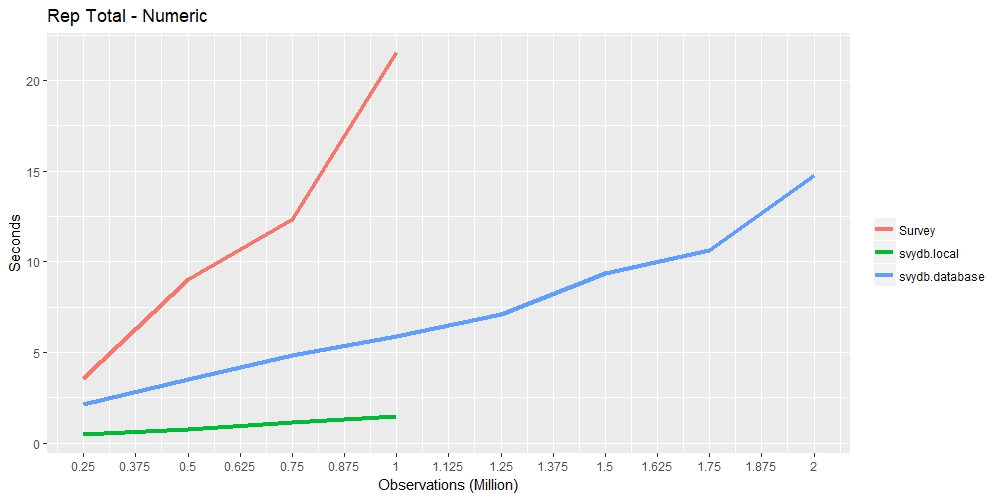
\includegraphics[scale = 0.6]{Latex/img/reptot-r.jpeg}
    \caption{Replicate total time comparison - Numeric}
    \label{fig:reptot-r}
\end{figure}
%--------------------------------------------------------------------------------------
\section{Mean - Replicate Weights}
\begin{figure}[H]
  \centering
    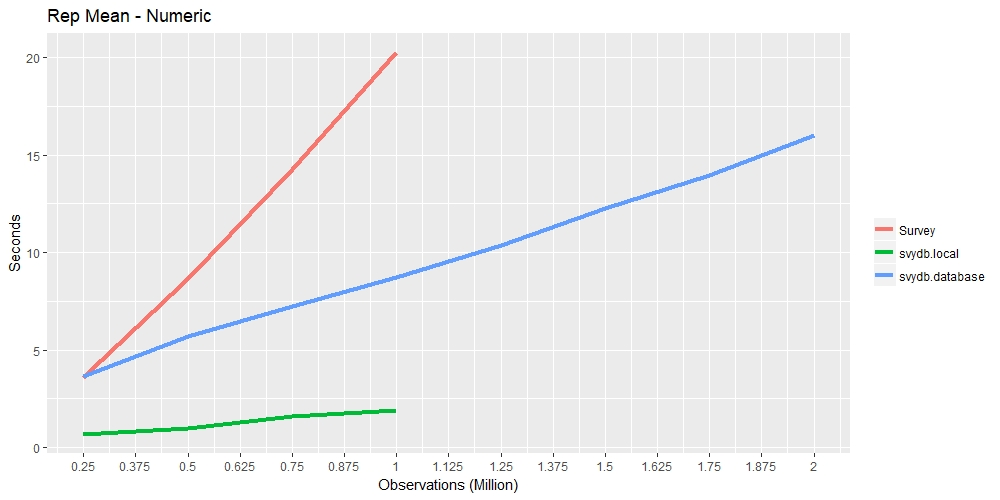
\includegraphics[scale = 0.6]{Latex/img/repmean-r.jpeg}
    \caption{Replicate mean time comparison - Numeric}
    \label{fig:repmean-r}
\end{figure}



%--------------------------------------------------------------------------------------
\section{Histogram}
\begin{figure}[H]
   \centering
    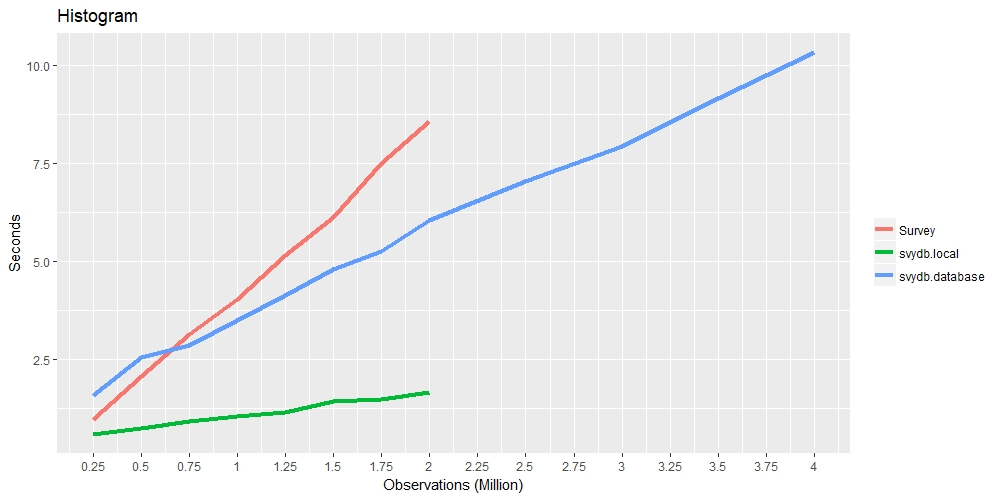
\includegraphics[scale = 0.6]{Latex/img/hist-r.jpeg}
    \caption{Histogram time comparison - Categorical}
    \label{fig:hist-r}
\end{figure}
%--------------------------------------------------------------------------------------
\section{Boxplot}
\begin{figure}[H]
   \centering
    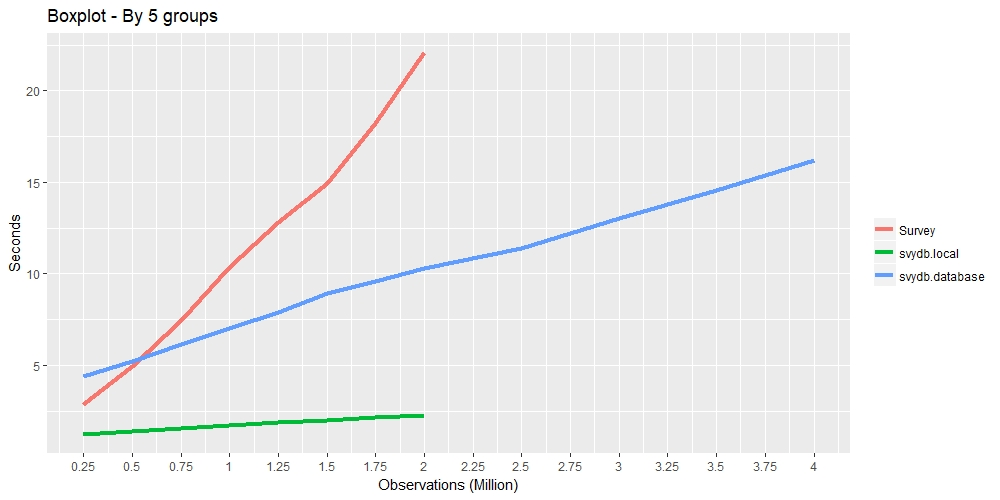
\includegraphics[scale = 0.6]{Latex/img/box-r.jpeg}
    \caption{Boxplot time comparison}
    \label{fig:box-r}
\end{figure}
%--------------------------------------------------------------------------------------
\section{Hexagon Binning}
\begin{figure}[H]
   \centering
    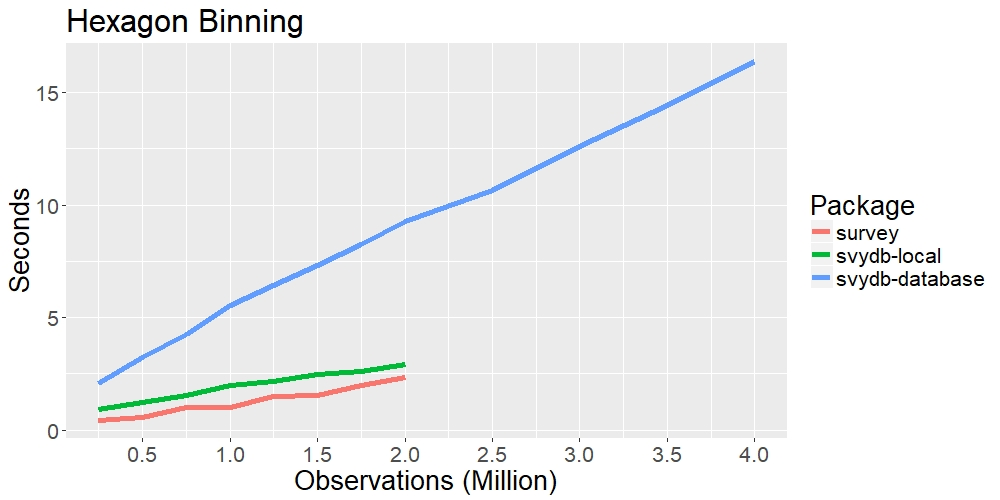
\includegraphics[scale = 0.6]{Latex/img/hex-r.jpeg}
    \caption{Hexagon Binning time comparison}
    \label{fig:hex-r}
\end{figure}
%--------------------------------------------------------------------------------------

\newpage

\section{Time Comparison}

In general, using {\bf svydb} with local data sets is always faster than both {\bf svydb} with data sets in a database or with the {\bf survey} package, except for computing the survey tables (\autoref{fig:table-r}) and hexagon binning (\autoref{fig:hex-r}), where the times were similar for survey tables and hexagon binning was always about 0.5 seconds slower.\\

In terms of data sets in a database, If using {\bf svydb} with local data sets is faster than the {\bf survey} package then the time it takes to compute survey statistics in a database with {\bf svydb} is predicted to be faster than the {\bf survey} package if the data set is large enough. When the data set gets larger, the increase in time for the {\bf survey} package is almost always larger than {\bf svydb}. In some cases with data sets up to two million observations, {\bf svydb} is already faster. \\

Most of the time we can see that {\bf svydb} with data sets in memory is the fastest, followed by the {\bf survey} package, and {\bf svydb} with data sets in a database is always the slowest. The reason is that it takes time for the computer to communicate with the database, as in telling it what to do and collecting the results. However, if the data sets are too large and cannot be fitted into memory, {\bf svydb} would be useful.\\

Some functions are just a replicate of another function but with more iterations and more features. For example, within {\bf svydbboxplot()} (\autoref{fig:box-r}), {\bf svydbquantile()} (\autoref{fig:quantile-r}) is called to obtain the quantiles, {\bf svydbhist()} (\autoref{fig:hist-r}) calls {\bf svydbmean()} (\autoref{fig:meannum-r}, \autoref{fig:meancat-r}) to obtain the proportions of each cut, and {\bf svydbreptotal()} (\autoref{fig:reptot-r}) is computed similarly to {\bf svydbtotal()} (\autoref{fig:totnum-r}, \autoref{fig:totcat-r}) but with more iterations with different sets of weights. Therefore, their computation time would be similar across different sizes of data set but with some sort of a scale factor.\\

Regression (\autoref{fig:lm-r}) is the most interesting, though the slope of the line for {\bf svydb.database} seems to be decreasing at 1.75 million observations, it is still around 1 to 1.5 seconds slower than the {\bf survey} package at the two million observations mark. Since matrix operations are not supported in a database, to get the result of a matrix multiplication is to calculate it row by row which would be slow. Therefore {\bf svydb.database} would only be expected to be faster than the {\bf survey} package if the data set is large enough, or if the model contains enough explanatory variables which results in an unfeasible matrix operation.\\

Though it seems as if {\bf svydb} is faster in most cases, but the structure of the {\bf survey} package is more complex, and what it can do is outside the capability of {\bf svydb}, for example, handling missing values, post-stratification and log models. At this stage it is unclear how much faster the {\bf survey} package would be if was only computing statistics that are implemented in {\bf svydb}.











